\documentclass[a4paper, 12pt, oneside]{book}

\pagestyle{myheadings}

\usepackage[T1]{fontenc}
\usepackage{ae}
\usepackage[utf8]{inputenc}
\usepackage[brazilian]{babel}
\usepackage{graphicx}
\usepackage[hyphens]{url}
\usepackage{hyperref}
\usepackage{physics}
\usepackage[export]{adjustbox}
\usepackage{float}

\linespread{1.5} 
\setlength{\hoffset}{-1in}
\setlength{\oddsidemargin}{3.0cm} 
\setlength{\textwidth}{160mm} 
\setlength{\parindent}{1.25cm} 
\setlength{\voffset}{-1in}
\addtolength{\voffset}{2.0cm}
\setlength{\topmargin}{0.0cm}
\setlength{\headheight}{5mm}
\setlength{\headsep}{5mm}
\setlength{\textheight}{247mm} 

%%%%%% COMPLETAR DADOS AQUI %%%%%%%%%%%
\def\titulo{Simulando Algoritmos Quânticos em um
Computador Clássico}
\def\tituloEN{Simulating Quantum Algorithms in a clássical
Computer}
\def\nome{Igor Valente Blackman}
\def\ano{2017}

\begin{document}

%%%%%%%%%%%%%%%%%%%%%%%%%%%%%%%%%%%%%%%%%%%%%%%
%     CAPA

\begin{titlepage}
 \noindent 
 \rule{\textwidth}{1ex} \\ [1ex]
 \begin{center}
  \begin{minipage}{0.15\textwidth}
   
\includegraphics[width=1\textwidth]{./logoUFF.png} 
  \end{minipage}
  \begin{minipage}{0.65\textwidth}
   \centering
   {\large \textsc{Universidade Federal Fluminense} } \\ [1.5ex]
   {\large \textsc{Instituto de Computação} } 
  \end{minipage}
  \begin{minipage}{0.15\textwidth}
   
\includegraphics[width=1\textwidth]{./logoIC.png}
  \end{minipage}
    
  \vfill
  {\Huge \textbf{\titulo}} \vfill
  {\huge \nome} \\ [25ex]
  {\large NITERÓI - RJ} \\ [1.5ex]
  {\large \ano}
 \end{center}\vspace{1ex}
 \rule{\textwidth}{1ex}
\end{titlepage}

%%%%%%%%%%%%%%%%%%%%%%%%%%%%%%%%%%%%%%%%%%%%%%%
%    CONTRA - CAPA

\begin{titlepage}
  \begin{center}
    \Large{\textsc{Universidade Federal Fluminense} \\
           \textsc{Instituto de Computação} \\ 
           \textsc{Departamento de Ciência da Computação} 
          }
    \par\vfill
    \LARGE{\nome}
    \par\vfill
    \LARGE{\titulo}
    \par\vfill
    \Large{NITERÓI - RJ \\
    \ano}
  \end{center}
\end{titlepage}

\pagenumbering{roman}
\setcounter{page}{2}

%%%%%%%%%%%%%%%%%%%%%%%%%%%%%%%%%%%%%%%%%%%%%%%
%    FOLHA DE ROSTO

\begin{center}

\MakeUppercase{\nome}

\vfill

\MakeUppercase{\titulo}

\vspace{3.0cm}

\begin{flushright}
\begin{minipage}{0.50\textwidth}

Trabalho submetido ao Curso de Bacharelado em Ciência da Computação da Universidade Federal Fluminense como requisito parcial para a obtenção do título de Bacharel em Ciência da Computação.

\end{minipage}
\end{flushright}

\vspace{3.0cm}

Orientadora: Profa. Dra. Karina Mochetti de Magalhães

\vfill

Niterói - RJ \\
\ano

\end{center}

\newpage

%%%%%%%%%%%%%%%%%%%%%%%%%%%%%%%%%%%%%%%%%%%%%%%%%%%%%    FICHA CATALOGRÁFICA

\newpage

%%%%%%%%%%%%%%%%%%%%%%%%%%%%%%%%%%%%%%%%%%%%%%%%%%%%%    FOLHA DE APROVAÇÃO

\newpage

%%%%%%%%%%%%%%%%%%%%%%%%%%%%%%%%%%%%%%%%%%%%%%%%%%%%%    DEDicatória

\begin{flushright}
\begin{minipage}{0.5\textwidth}

\vspace{15.0cm}

\emph{
Dedico este trabalho aos meus pais e a toda minha família que me apoiaram desde sempre e sem eles não seria o que sou e onde cheguei.
}

\emph{Ao curso de Ciência da Computação na Universidade Federal Fluminense, aos professores e aos colegas de faculdade que conheci ao longo desses anos.}

\end{minipage}
\end{flushright}

%%%%%%%%%%%%%%%%%%%%%%%%%%%%%%%%%%%%%%%%%%%%%%%%%%%%%    AGRADECIMENTOS

\chapter*{Agradecimentos}
\addcontentsline{toc}{chapter}{Agradecimentos}

\thispagestyle{myheadings}

\noindent

À professora Karina Mochetti, pela orientação, revisão, cobrança, paciência e coragem de me aceitar como orientando.

\ \\ 

Aos meus pais que me ajudaram no que era possivel para eles, sempre me incentivando não importando o que fosse.

\ \\ 

À minha irmã...bom, esquece.

\ \\ 

Aos meus amigos Pumbas pelo incentivo, auxílio e testes sempre que necessário não importando a hora.

%%%%%%%%%%%%%%%%%%%%%%%%%%%%%%%%%%%%%%%%%%%%%%%%%%%%%    RESUMO

\chapter*{Resumo}
\addcontentsline{toc}{chapter}{Resumo}

\thispagestyle{myheadings}

A construção de um computador quântico terá impactos profundos em várias áreas, tais como Física, Matémática e, especialmente, a Ciência da Computação. As dificuldades práticas em se construir um computador quântico são muitas, logo não é possível prever quando ou mesmo se um computador quântico será construído. Apesar disso, a teoria na área da computação quântica vem evoluindo fortemente e para auxiliar na análise desses algoritmos pode ser essencial a criação de um simulador quântico de fácil acesso. Esse simulador utilizaria um computador clássico para realizar os trabalhos de um computador quântico, simulando o entrelaçamento e a sobreposição em bits clássicos e realizando uma estimativa de tempo gasto num computador quântico. O objetivo desse trabalho é realizar a implementação desse simulador de algoritmos quânticos.

\ \\

Palavras-chave: quântica, circuito, simulador quântico, aplicação web. 

%%%%%%%%%%%%%%%%%%%%%%%%%%%%%%%%%%%%%%%%%%%%%%%%%%%%%    ABSTRACT

\chapter*{Abstract}
\addcontentsline{toc}{chapter}{Abstract}

\thispagestyle{myheadings}

The construction of a quantum computer will have deep impacts in several areas, such as Physics, Mathematics, and especially Computer Science. There are several practical difficulties in building a quantum computer, so it is not possible to predict when or even if a quantum computer will be built. Nevertheless, the theory in the Quantum Computing field is evolving strongly and to assist in the analysis of these algorithms can be essential to create a quantum simulator. This simulator would be implemented in a classic computer, performing the work of a quantum computer, emulating the superposition and entanglement in classical bits with an estimate of efficiency. Therefore, the goal of this work is to implement a simulator for quantum algorithms.

\ \\

Keywords: quantum, quantum simulator, circuit, web application.

%%%%%%%%%%%%%%%%%%%%%%%%%%%%%%%%%%%%%%%%%%%%%%%%%%%%%    SUMáRIO

\tableofcontents

\thispagestyle{myheadings}

%%%%%%%%%%%%%%%%%%%%%%%%%%%%%%%%%%%%%%%%%%%%%%%%%%%%%    LISTA DE FIGURAS

\listoffigures
\addcontentsline{toc}{chapter}{Lista de Figuras}

\thispagestyle{myheadings}

%%%%%%%%%%%%%%%%%%%%%%%%%%%%%%%%%%%%%%%%%%%%%%%%%%%%%    LISTA DE TABELAS

%\listoftables
%\addcontentsline{toc}{chapter}{Lista de Tabelas}

%\thispagestyle{myheadings}

%%%%%%%%%%%%%%%%%%%%%%%%%%%%%%%%%%%%%%%%%%%%%%%%%%%%%    TEXTO

\pagebreak
\pagenumbering{arabic}

\chapter{Introdução}
\thispagestyle{empty}

A computação quântica aproveita a possibilidade de superposição de estados das partículas subatômicas~\cite{wiredQC}. Em um computador normal, que chamaremos de clássico, um bit é um simples pedaço de informação que possui apenas dois estados, 0 ou 1. Para representar tal informação um computador deve conter algum tipo de sistema físico com dois estados distintos para associar aos valores como, por exemplo, um switch que pode estar fechado (1) ou aberto (0)~\cite{mermin}.

Computadores quânticos, por sua vez, utilizam bits quânticos ou ``qubits'', que também possuem dois estados, entretanto, diferente do bit clássico, qubits podem armazenar muito mais informação já que eles podem existir em qualquer sobreposição desses valores, 0, 1, ou ambos ao mesmo tempo~\cite{wiredQC}. 

No mundo da mecânica quântica os eventos são governados por probabilidades. Um átomo radioativo, por exemplo, pode enfraquecer emitindo um elétron, ou não. É possível preparar um experimento de tal forma que exista uma chance exata de 50\% de que um dos átomos de um pedaço de material radioativo caia em um determinado tempo~\cite{gribbin}.

Pode-se tomar como exemplo o experimento teórico do ``Gato de \textit{Schrödinger}''. São colocados um gato, um frasco de veneno e uma fonte de radiação em uma caixa selada. Se um monitor interno (ex. Contador Geiger) detecta radiação, o frasco é quebrado soltando o veneno, matando o gato. No mundo quântico existe uma chance de 50\% de o gato estar morto, e sem olhar dentro da caixa não podemos dizer se o gato está vivo ou morto. Segundo a teoria, nenhuma das duas possibilidades tem qualquer realidade a menos que seja observada~\cite{gribbin}. Isso se equivale para o qubit, ele pode ser 0 ou 1 ao mesmo tempo mas quando ele é observado ele deixa de ser um bit quântico e passa a ser um bit clássico, ou seja, só pode ser 0 ou 1.

Outra representação de um qubit pode ser uma esfera imaginária, ilustrada na Figura~\ref{fig:bloch}, onde um bit clássico pode estar apenas em um dos pólos da esfera e o qubit, bit quântico, pode estar em qualquer ponto da esfera. Assim qubits podem armazenar uma quantidade muito maior de informação que um bit clássico.

\begin{figure}[H]
\centering
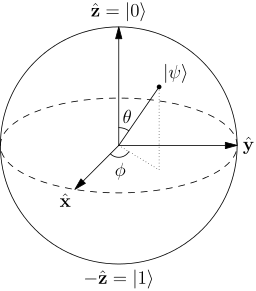
\includegraphics[scale=0.5]{bloch_sphere.png}
\caption{Esfera de Bloch}
\label{fig:bloch}
\end{figure}
%imagem retirada da wikipedia

\section{Motivação e Objetivo}

A computação quântica é uma área de pesquisa muito relevante, pois utiliza elementos de áreas importantes como a Física, a Matemática e a Engenharia. Apesar de ainda não ser possível prever quando ou mesmo se um computador quântico será construído, caso isto ocorra serão gerados grandes impactos em todas essas áreas. Em um computador quântico, os sistemas não devem ter interações físicas que não estejam sob o controle total e completo do programa. Diferente de como ocorre em um computador clássico, interações físicas não controladas introduziriam interrupções potencialmente catastróficas na operação de um computador quântico, o que resulta em uma dificuldade na construção do mesmo. 

Entretanto, os benefícios que podem ser gerados com a construção de um computador quântico vão muito além do que os pesquisadores podem imaginar. Para os cientistas da computação, o mais impressionante na computação quântica é a eficiência alcançada por seus algoritmos, algo não possível na teoria clássica da complexidade computacional. O tempo de execução de algumas tarefas em um computador quântico cresce de forma muito mais lenta com o tamanho da entrada do que em um computador clássico, como exemplo temos o algoritmo clássico de busca que possui complexidade O(N) e o algoritmo quântico de busca, conhecido por Algoritmo de Grover, possibilita que esse método de busca chegue a complexidade O$(\sqrt{N})$~\cite{grover}. 

Neste trabalho apresentamos a implementação de um simulador de circuitos quânticos que utiliza um computador clássico para executar os algoritmos quântico. Assim, características quânticas como o entrelaçamento e a sobreposição serão realizadas em bits clássicos o que resultará num gasto de tempo maior. Por isso, o simulador também gera uma estimativa de tempo gasto a partir das portas quânticas, emulando o que seria obtido por um computador quântico caso ele seja construído; as portas e o tempo gasto em cada uma são dados pelo usuário. O simulador é uma ferramenta online e dispõe de arraste das portas quânticas para formação dos circuitos com o intuito de facilitar a interação com o usuário, ter uma interface simples e como diferencial gerar uma estimativa de tempo gasto.

\section{Trabalhos Relacionados}

Nesta sessão mostramos alguns simuladores que existem e quais suas vantagens e desvantagens.

\subsection{Quantum - Davy Wybiral}

Existe um simulador online desenvolvido por Davy Wybiral de Austin Texas, \textit{Quantum} ou como está no projeto dele do Git \textit{Quantum Circuit Simulator}~\cite{davyw}. O projeto foi disponibilizado no Git em Janeiro de 2017~\cite{gitdavyw}. Davy Wybiral utiliza o Canvas para gerar toda a parte gráfica dos circuitos e menus, e javascript para toda a parte de cálculo. O simulador não possui nenhum tipo de documentação e tem uma interface bem simples com um menu superior onde existem algumas opções e uma área com as portas quânticas que podem ser adicionadas nos circuitos e ter a quantidade dos mesmos alterada, como pode ser visto na Figura~\ref{fig:davyw}.

\begin{figure}[H]
\centering
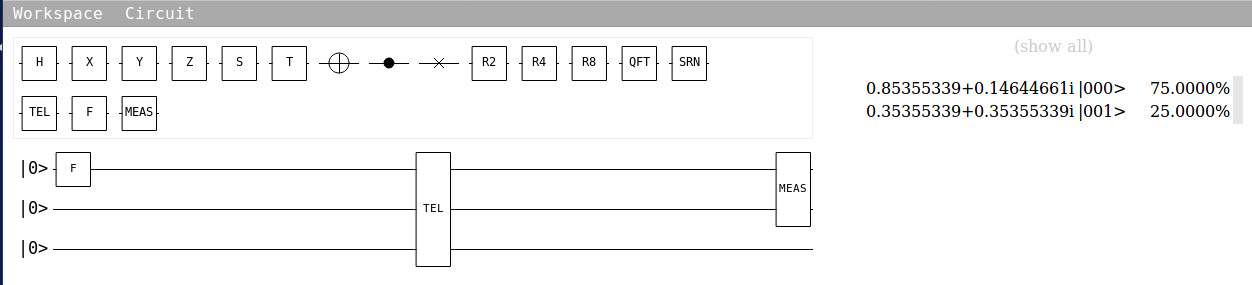
\includegraphics[scale=0.36]{davyw.jpg}
\caption{Simulador quântico de Davy Wybiral}
\label{fig:davyw}
\end{figure}

A montagem do circuito funciona com a seleção de uma das portas e após isso basta clicar nos circuitos para adicionar a porta selecionada. Pode-se deletar uma porta clicando com o botão direito. Nos casos de portas de 2-bits é necessário que haja uma ação de clique e arraste onde o clique seleciona a posição do bit de controle e o largar selecionar a porta. Existe também a possibilidade de arrastar com uma porta de 1-bit selecionada o que adiciona a mesma em diversos circuitos.

Para efetuar o cálculo do circuito basta pressionar a tecla Enter ou selecionar no menu a opção \textit{Evaluate}. O resultado é mostrado ao lado direito com todas as possibilidades possíveis e suas respectivas probabilidades.

\subsection{IBM Q experience}

IBM \textit{Quantum experience} (IBM Q experience) tem como objetivo ajudar no aprendizado sobre o mundo quântico lendo o guia de usuário da ferramenta, realizando seus próprios experimentos, simulando-os e executando-os no processador quântico através do IBM Cloud~\cite{ibmq}.

O IBM Quantum Experience é composto por:
\begin{itemize}
\item um conjunto de tutoriais que vão desde simples experimentos com únicos qubits a experimentos mais complexos com múltiplos qubits;
\item o \textit{Quantum Composer}, uma interface gráfica para criação de circuitos quânticos, os quais eles chamam de \textit{quantum score};
\item um simulador que testa seus \textit{quantum scores};
\item acesso a um processador quântico que roda no laboratório da IBM \textit{Quantum Computing}, onde os seus quantum scores serão executados;
\item a \textit{quantum community} onde \textit{quantum scores}, ideias e experiências são compartilhadas e discutidas.
\end{itemize}

No \textit{Quantum Composer}, interface gráfica para construção de circuitos quânticos, logo de inicio existe a opção de executar em um processador quântico ``real'' ou em um processador quântico customizado. Na segunda opção as portas podem ser colocadas em qualquer lugar enquanto na primeira a topologia é definida pelo dispositivo físico no qual está sendo executado no laboratório.

\begin{figure}[H]
\centering
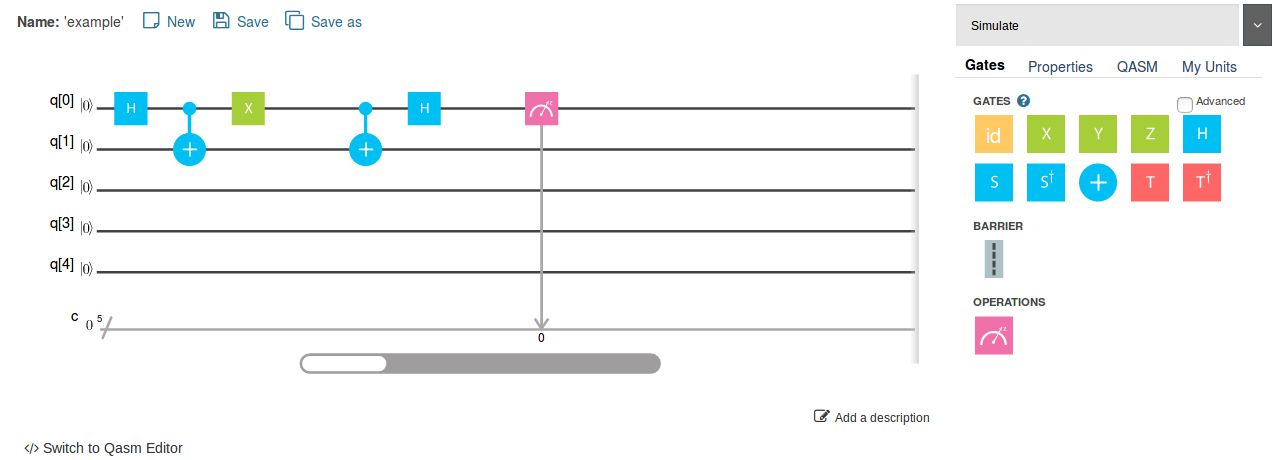
\includegraphics[scale=0.36]{ibmq.png}
\caption{Interface gráfica \textit{Quantum Composer} do IBM Q Experience}
\label{fig:ibmq}
\end{figure}

Como pode-se notar na Figura~\ref{fig:ibmq} a interface é composta pela área do circuito na parte esquerda da tela com cada linha sendo equivalente a um qubit. Já na parte direita existem as portas que podem ser arrastadas para montar o circuito, e caso o usuário clique em alguma porta dentro do circuito uma explicação sobre a mesma é mostrada nesta área.

\subsection{Quirk - Craig Gidney}

O projeto teve seu início em Março de 2014, mas não teve commits após o mês de criação. Em Novembro do mesmo ano, 2014, voltou a ter commits e entre Março de 2016 e Novembro de 2016 teve a maior concentração de commits, 647 dos 1006 totais. O projeto ainda vem sendo atualizado sendo o commit mais recente do dia 29 de Abril de 2017~\cite{gitquirk}. Craig Gidney, desenvolvedor do Quirk, explica que decidiu criar o simulador porque ficou interessado em computação quântica e pelo fato de ter lido ``\textit{Media for Thinking the Unthinkable}'' de Bret Victor onde ele menciona benefícios do \textit{feedback} imediato em relação ao entendimento e produtividade. Craig diz não ter achado nenhum simulador de circuitos quânticos que passasse essa experiência de ``manipulação direta''~\cite{quirk}. Foi desenvolvido utilizando Webgl. Na Figura~\ref{fig:quirk} pode-se ver uma captura de tela do simulador.

\begin{figure}[hbtp]
\centering
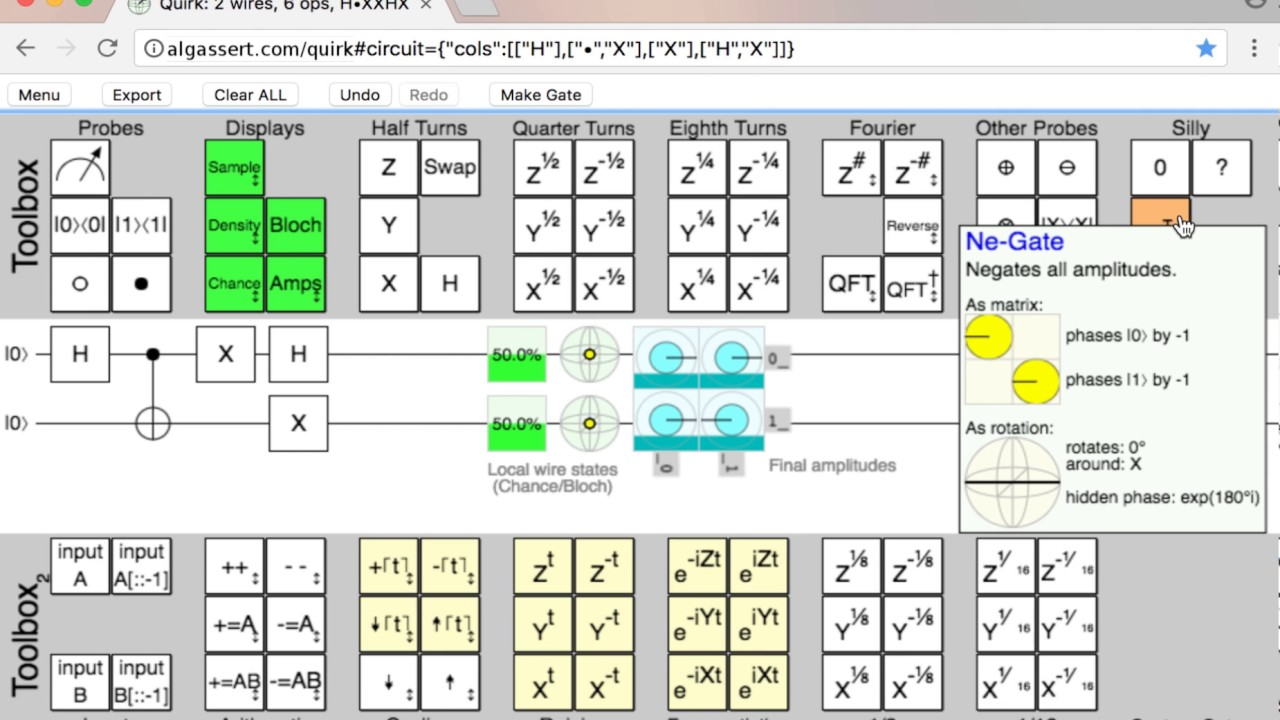
\includegraphics[scale=0.36]{quirk.jpg}
\caption{Simulador quântico Quirk de Craig Gidney}
\label{fig:quirk}
\end{figure}

Craig faz comparações com alguns simuladores como, por exemplo, o já mencionado de Davy Wybiral e o IBM \textit{Quantum Experience}. Ele também menciona alguns outros como \textit{Quantum Computing Playground} e Microsoft's LIQ Ui|>.

O simulador Quirk é composto por um menu que possui opções de carregar alguns exemplos de circuitos já prontos, exportar o circuito montado, desfazer ou refazer alguma alteração e inclusive criar porta. Ele possui uma área com as opções de portas a serem utilizadas no circuito, formas de mostrar o resultado e mais diversas opções. Algumas vantagens desse simulador são: as portas são colocadas da forma ``arrastar e soltar'', o resultado é mostrado a todo momento não havendo a necessidade de se apertar um botão para isso, e é possível adicionar mais bits ao circuito dinamicamente com o arrastar de uma das portas para além da linha do último bit.

\subsection{Comparação}

O nosso simulador tem como objetivo ser simples como o Quantum do Davy Wybiral entretanto com mais funcionalidades, como o arraste das portas para construção do circuito, existente nos dois outros simuladores. Menos poluído que o Quirk do Craig Gidney. E gerando uma estimativa de tempo gasto com a passagem dos tempos das portas quânticas pelo usuário, uma funcionalidade que nenhum dos três disponibiliza.

\section{Organização do Texto}

Este trabalho está divido da seguinte forma: a Seção 2 são apresentados alguns tópicos sobre circuito quântico que são utilizados ao longo do projeto; na Seção 3 é apresentada a escolha das ferramentas utilizadas para o desenvolvimento do simulador, expondo a teoria e os frameworks existentes atualmente; a Seção 4 apresenta como a solução foi desenvolvida e como resultado o código gerado; e por final na Seção 5 são apresentadas as conclusões e trabalhos futuros.

%%%%%%%%% Circuitos Quanticos
\chapter{Circuito Quântico}

\section{Circuitos digitais}
Os circuitos lógicos clássicos são formados por portas como AND, OR e NOT que recebem uma sequência de valores binários 0 e 1. Ao passar pelas portas é gerada uma saída que representa a entrada transformada pelo circuito, como ilustrado na Figura~\ref{fig:classiccircuit}~\cite{nielsen}.

\begin{figure}[H]
\centering
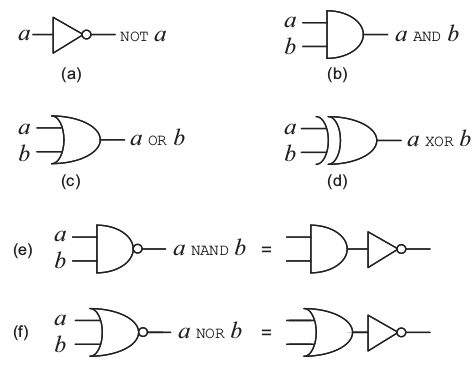
\includegraphics[scale=0.5]{classiccircuit.png}
\caption{Exemplos de portas clássicas}
\label{fig:classiccircuit}
\end{figure}
%peguei do livro do Nielsen

\section{Qubit}
Dentro do espaço vetorial bidimensional os únicos vetores clássicos são os dois vetores ortogonais $\ket{0}$ e $\ket{1}$, visto que esses são os únicos dois estados que um bit clássico pode ter. Já um bit quântico, ou seja, um qubit possui um estado associado $\ket{\Psi}$ que pode ser qualquer vetor unitário dentro do espaço vetorial bidimensional abrangido por $\ket{0}$ e $\ket{1}$ sobre os números complexos, ou seja, um vetor composto de dois números complexos que chamaremos de a e b, como pode se notar em~\eqref{eq1}.
\begin{equation} \label{eq1} 
\ket{\Psi} = a\ket{0} + b\ket{1} = \mqty(a\\b).
\end{equation}

Como a única exigência de $\ket{\Psi}$ é ser um vetor unitário dentro do espaço vetorial complexo, a condição de normalização se aplica a ele, tendo assim~\eqref{eq2}~\cite{mermin}
\begin{equation}\label{eq2}
\abs{a}^2 + \abs{b}^2 = 1,
\end{equation}

O estado $\ket{\Psi}$ define uma superposição dos estados $\ket{0}$ e $\ket{1}$ com amplitudes \textit{a} e \textit{b}. Se a for 1, por exemplo, temos o caso especial onde o estado do qubit é igual a $\ket{0}$. Respectivamente, temos o estado $\ket{1}$ caso b seja 1.

Ao ser medido os elementos $\abs{a}^2$ e $\abs{b}^2$ são, respectivamente, a probabilidade de que o qubit seja $\ket{0}$ e $\ket{1}$, logo 
\begin{align*} 
  \ket{0} = \mqty(1\\0) ,\hspace{2cm} 
  \ket{1} = \mqty(0\\1).
\end{align*}


\section{Entrelaçamento}
Assim como o estado geral de um único qubit é qualquer superposição normalizada dos dois possíveis estados clássicos~\eqref{eq1}, o estado geral de $\ket{\Psi}$ nos possibilita associar com dois qubits em qualquer superposição dos quatro estados clássicos,
\begin{equation}\label{eq3}
\ket{\Psi}_2 = a\ket{00} + b\ket{01} + c\ket{10} + d\ket{11} = \mqty(a\\b\\c\\d)
\end{equation}
\begin{align*}
  \ket{00} = \mqty(1\\0\\0\\0) \hspace{1cm} 
  \ket{01} = \mqty(0\\1\\0\\0) \hspace{1cm} 
  \ket{10} = \mqty(0\\0\\1\\0) \hspace{1cm} 
  \ket{11} = \mqty(0\\0\\0\\1)
\end{align*}

Assim os valores das quatro amplitudes devem seguir a condição de normalização, onde
\begin{equation}\label{eq4}
\abs{a}^2 + \abs{b}^2 + \abs{c}^2 + \abs{d}^2 = 1
\end{equation}

Generalizando para \textit{n} qubits o estado geral pode ser qualquer superposição dos $2^n$ estados clássicos, com amplitudes cujo quadrado somam a unidade:
\begin{align*}
\ket{\Psi} = \sum_{0\leq x<2^n} \alpha_x\ket{x}_n \\
\sum_{0\leq x<2^n} \abs{\alpha_x}^2 = 1.
\end{align*}
No contexto de computação quântica, o conjunto de $2^n$ estados clássicos, isto é, todos os possíveis produtos tensores de \textit{n} qubits $\ket{0}$ e $\ket{1}$ é chamado de base clássica. Os estados que caracterizam \textit{n} bits clássicos, estados de base clássica, são um conjunto bem limitado dos estados de \textit{n} qubits, os quais podem ser qualquer superposição com coeficientes complexos desses estados de base clássica~\cite{mermin}.

Se tivermos dois qubits, um no estado $\ket{\Psi} = a'\ket{0} + b'\ket{1}$ e outro no estado $\ket{\Phi} = c'\ket{0} + d'\ket{1}$, então o estado de 2-qubits $\ket{\Psi}$ do par é o produto tensorial dos estados individuais,
\begin{equation}\label{eq7}
\ket{\Psi}_2 = \ket{\Psi}\otimes\ket{\Phi} 
= a'c'\ket{00} + a'd'\ket{01} + b'c'\ket{10} + b'd'\ket{11}
= \mqty(a' \vdot c'\\a' \vdot d'\\b' \vdot c'\\b' \vdot d')
\end{equation}\
Com \eqref{eq7} e a condição de normalização temos
\begin{align*}
\abs{a' \vdot c'}^2 + \abs{a' \vdot d'}^2 + \abs{b' \vdot c'}^2 + \abs{b' \vdot d'}^2 \\
\abs{a'}^2 \vdot \abs{c'}^2 + \abs{a'}^2 \vdot \abs{d'}^2 + \abs{b'}^2 \vdot \abs{c'}^2 + \abs{b'}^2 \vdot \abs{d'}^2 \\
\abs{a'}^2 \vdot (\abs{c'}^2 + {d'}^2) + \abs{b'}^2 \vdot (\abs{c'}^2 + \abs{d'}^2) \\
\abs{a'}^2 \vdot 1 + \abs{b'}^2 \vdot 1 \\
\abs{a'}^2 + \abs{b'}^2 = 1
\end{align*}

Note que um estado geral de 2-qubit \eqref{eq3} é da forma especial \eqref{eq7} se e somente se $a'\vdot d'=b'\vdot c'$. Como as quatro amplitudes seguem a condição de normalização \eqref{eq4}, essa relação não se mantém, e o estado geral de 2-qubit é diferente do estado geral de 2 bits clássicos, ele não é um produto \eqref{eq7} de dois estados de 1-qubit. O mesmo é verdade para estados de n-qubits. Enquanto o estado geral de n bits clássicos é um dos $2^n$ produtos de $\ket{0}$s e $\ket{1}$s, o estado geral de n-qubits é a superposição desses $2^n$ produtos e não pode ser expresso como um produto de qualquer conjunto de estados de 1-qubit~\cite{mermin}. Esse não produto de estados de dois ou mais qubits é chamado de entrelaçamento.

\section{Portas quânticas}
Assim como um computador clássico é formado de circuitos com portas lógicas, um computador quântico também é formado por circuitos. Porém, este último possui portas quânticas~\cite{nielsen}, que definem as operações básicas que podemos realizar em qubits. Essas portas podem ser representadas graficamente através de circuitos, como visto na Figura~\ref{fig:portaQuantica}, ou matematicamente por matrizes, como visto na equação~\eqref{eqPortas}.
\begin{equation}\label{eqPortas}
\ket{\Psi'} =  U\ket{\Psi}
\end{equation}

\begin{figure}[H]
\centering
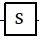
\includegraphics[scale=0.75]{s.jpg}
\caption{Porta quântica}
\label{fig:portaQuantica}
\end{figure}

Uma porta quântica deve sempre ser representada por uma matriz unitária pois ao multiplicar o vetor pela matriz a norma do vetor deve ser mantida.

\subsection{Identidade} \label{sec:identidade}
A operação Identidade quântica mantém os valores iniciais do qubit, representada graficamente pela Figura~\ref{fig:I} e pela matriz~\eqref{eqI}. Ela é trivial e não realiza qualquer modificação no qubit.
\begin{equation}\label{eqI}
I =  \mqty(1&0\\0&1)
\end{equation}

\begin{figure}[H]
\centering
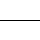
\includegraphics[scale=0.75]{line.jpg}
\caption{Porta quântica Identidade}
\label{fig:I}
\end{figure}

\begin{align*}
I\ket{\Psi} = \mqty(1&0\\0&1)\mqty(a\\b) = \mqty(1 \vdot a+0 \vdot b \\0 \vdot a+1 \vdot b) = \mqty(a\\b) = \ket{\Psi'}
\end{align*}

\subsection{NOT} 
Considerando as portas de um único bit, a única porta clássica é a porta NOT a qual faz com que os bits 0 e 1 se invertam. Imagine o mesmo processo que recebe o estado $\ket{0}$ e retorna o estado $\ket{1}$, e vice versa. Este processo seria um bom candidato para a porta quântica análoga a NOT clássica. Entretanto, especificando a ação sobre os estados $\ket{0}$ e $\ket{1}$ não nos diz nada sobre o que aconteceria sobre a superposição dos mesmos. Na verdade, a porta quântica NOT age linearmente, ou seja, recebe o estado $a\ket{0} + b\ket{1}$ e retorna $b\ket{0} + a\ket{1}$, assim invertendo as amplitudes do qubit~\cite{nielsen}. A porta quântica NOT pode ser representada graficamente pela Figura~\ref{fig:not} e um outro modo conveniente de representá-la é em forma de matriz \eqref{eq2x}.

\begin{equation}\label{eq2x}
X =  \mqty(0&1\\1&0)
\end{equation}

\begin{figure}[H]
\centering
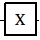
\includegraphics[scale=0.75]{x.jpg}
\caption{Porta quântica NOT}
\label{fig:not}
\end{figure}

Com o estado $\ket{\Psi} = \mqty(a\\b)$, podemos aplicar \eqref{eq2x} e teremos
\begin{align*}
X\ket{\Psi} = \mqty(0&1\\1&0)\mqty(a\\b) = \mqty(0 \vdot a+1 \vdot b \\1 \vdot a+0 \vdot b) = \mqty(b\\a) = \ket{\Psi'}
\end{align*}

\subsection{Y e Z} 
Diferentemente da computação clássica, na qual só existe uma porta de um bit, na computação quântica existem várias portas de um único qubit. Como, por exemplo, as operações Y e Z, que são representadas graficamente pelas Figuras \ref{fig:y} e \ref{fig:z}, e matricialmente por \eqref{eqY} e \eqref{eqZ} respectivamente. Essas operações são análogas a operação NOT se pensarmos na representação do estado de um qubit como uma esfera, ilustrado pela esfera de Bloch na Figura \ref{fig:bloch}. A operação NOT é equivalente a rotação da esfera no eixo X em $\pi$ radianos e análogamente, as operações Y e Z são rotações de $\pi$ radianos nos eixos Y e Z, respectivamente.

\begin{equation}\label{eqY}
Y =  \mqty(0&-i\\i&0)
\end{equation}

\begin{figure}[H]
\centering
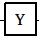
\includegraphics[scale=0.75]{y.jpg}
\caption{Porta quântica Y}
\label{fig:y}
\end{figure}

\begin{align*}
Y\ket{\Psi} = \mqty(0&-i\\i&0)\mqty(a\\b) = \mqty(0 \vdot a-i \vdot b \\i \vdot a+0 \vdot b) = \mqty(-bi\\ai) = \ket{\Psi'}
\end{align*}

\begin{equation}\label{eqZ}
Z =  \mqty(1&0\\0&-1)
\end{equation}

\begin{figure}[H]
\centering
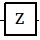
\includegraphics[scale=0.75]{z.jpg}
\caption{Porta quântica Z}
\label{fig:z}
\end{figure}

\begin{align*}
Z\ket{\Psi} = \mqty(1&0\\0&-1)\mqty(a\\b) = \mqty(1 \vdot a+0 \vdot b \\0 \vdot a-1 \vdot b) = \mqty(a\\-b) = \ket{\Psi'}
\end{align*}

\subsection{Hadamard} 
A porta Hadamard é uma operação fundamental na computação quântica e não possui uma operação clássica equivalente. Ela pode ser representada pela Figura~\ref{fig:H} ou pela matriz~\eqref{eqH}. Essa porta transforma os qubits bases $\ket{0}$ e $\ket{1}$ para um estado de sobreposição onde $\ket{0}$ e $\ket{1}$ possuem a mesma probabilidade. Se consideramos a esfera de Bloch ela seria equivalente a realizar essa operação sobre ela, isto é uma rotação da esfera no eixo Y de $90^o$ e em seguida uma rotação no eixo X de $180^o$, como é mostrado na Figura~\ref{fig:h_sphere}~\cite{nielsen}.

\begin{figure}[H]
\centering
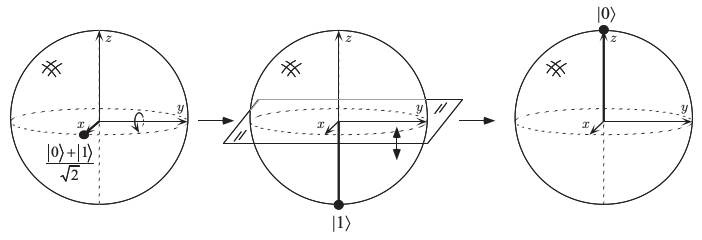
\includegraphics[scale=0.6]{h_sphere.png}
\caption{Esferas de Bloch da operação Hadamard}
\label{fig:h_sphere}
\end{figure}
%imagem pega do livro do Nielsen

\begin{equation}\label{eqH}
H =  \frac{1}{\sqrt{2}}\mqty(1&1\\1&-1)
\end{equation}

\begin{figure}[H]
\centering
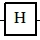
\includegraphics[scale=0.75]{h.jpg}
\caption{Porta quântica Hadamard}
\label{fig:H}
\end{figure}

Assim, para um qubit de probabilidade $\abs{a}^2$ e $\abs{b}^2$ teríamos um qubit resultante com probabilidades $\frac{(a+b)^2}{2}$ e $\frac{(a-b)^2}{2}$

\begin{equation}
H\ket{\Psi} = \frac{1}{\sqrt{2}}\mqty(1&1\\1&-1)\mqty(a\\b) = \frac{1}{\sqrt{2}}\mqty(1 \vdot a+1 \vdot b \\1 \vdot a-1 \vdot b) = \mqty( \frac{a+b}{\sqrt{2}} \\ \frac{a-b}{\sqrt{2}} ) = \ket{\Psi'}
\end{equation}

\subsection{CNOT} \label{sec:cnot}
A operação CNOT é uma porta de dois qubits conhecidos como controle e alvo, representada pela matriz~\eqref{eqCNOT} ou pela Figura~\ref{fig:CNOT}, na qual a linha de cima representa o qubit de controle e a de baixo o qubit alvo~\cite{mermin}. A porta CNOT funciona da seguinte maneira: dados dois qubits, $\ket{x}$ e $\ket{y}$, a matriz C mantém o valor de $\ket{y}$ caso $\ket{x}$ seja igual a $\ket{0}$ e caso $\ket{x}$ seja igual a $\ket{1}$ ela inverte o valor de $\ket{y}$, como é mostrado em~\eqref{eqFullCNOT}.
\begin{equation}\label{eqCNOT}
C =  \mqty(1&0&0&0\\0&1&0&0\\0&0&0&1\\0&0&1&0)
\end{equation}

\begin{figure}[H]
\centering
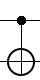
\includegraphics[scale=0.80]{cnot.png}
\caption{Porta quântica CNOT}
\label{fig:CNOT}
\end{figure}

Assim, para dois qubits entrelaçados, ela inverterá as amplitudes referentes aos qubits $\ket{10}$ e $\ket{11}$:

\begin{equation}\label{eqFullCNOT}
C\ket{\Psi} = \mqty(1&0&0&0\\0&1&0&0\\0&0&0&1\\0&0&1&0)\mqty(a\\b\\c\\d) = 
\mqty(1 \vdot a+0 \vdot b +0 \vdot c +0 \vdot d \\
	  0 \vdot a+1 \vdot b +0 \vdot c +0 \vdot d \\
	  0 \vdot a+0 \vdot b +0 \vdot c +1 \vdot d \\
	  0 \vdot a+0 \vdot b +1 \vdot c +0 \vdot d ) 
= \mqty(a\\b\\d\\c) = \ket{\Psi'}
\end{equation}

\subsection{Medição} \label{sec:medicao}
Outra porta importante é a de medição, que comumente é representada por um ``medido'', como pode ser observado na Figura~\ref{fig:medicao}. Essa operação converte um único qubit no estado $\ket{\Psi}=a\ket{0}+b\ket{1}$ em um bit clássico probabilístico, o qual é 0 com uma probabilidade de $\abs{a}^2$, ou 1 com uma probabilidade $\abs{b}^2$~\cite{mermin}. Para fazer essa diferenciação entre qubit e bit clássico em um circuito lógico quântico, um traço representa um qubit e um traço duplo um bit clássico.

Esta é uma porta trivial em um circuito clássico, normalmente nem representada, sendo uma das maiores diferenças entre circuitos quânticos e clássicos.

\begin{figure}[H]
\centering
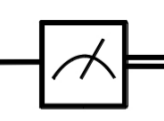
\includegraphics[scale=0.40]{medicao.png}
\caption{Porta quântica de medição}
\label{fig:medicao}
\end{figure}

\section{Operações em qubits entrelaçados}

Dados dois qubits $\ket{\Psi_1}$ e $\ket{\Psi_2}$ podemos fazer a operação $A$ em $\ket{\Psi_1}$ e $B$ em $\ket{\Psi_2}$ como $C$ se ambos estiverem entrelaçados formando um 2-qubit \eqref{eq:cab}.

\begin{align} \label{eq:cab}
C = A \otimes B
\end{align}

O produto tensorial pode ser expandido para matrizes em geral.

\begin{align*}
A \otimes B = \mqty(a_{11}\vdot B & a_{12}\vdot B & \hdots & a_{1n}\vdot B \\
  a_{21}\vdot B & a_{22}\vdot B & \hdots & a_{2n}\vdot B \\
  \vdots & \vdots & \hdots & \vdots \\
  a_{n1}\vdot B & a_{n2}\vdot B & \hdots & a_{nn}\vdot B \\
)
\end{align*}

Para qualquer operação em $\ket{\Psi_1}$ seja transformada em uma operação para um 2-qubit $\ket{\Psi_{12}}$, basta realizar o produto tensorial com a identidade em $\ket{\Psi_2}$ 
\begin{align} \label{eq:cai}
C = A \otimes I
\end{align}

\begin{align*}
A \otimes I (\ket{\Psi_1} \otimes \ket{\Psi_2} = \\
  (A\ket{\Psi_1}) \otimes (I\ket{\Psi_2}) = \\
  A\ket{\Psi_1} \otimes \ket{\Psi_2} = \\
  A(\ket{\Psi_1} \otimes \ket{\Psi_2})
\end{align*}

Agora no caso de duas operações transformadas, dadas as operações A em $\ket{\Psi_1}$ e B em $\ket{\Psi_2}$, temos $C = A\ket{\Psi_1} \otimes I\ket{\Psi_2}$ e $B_{12} = I\ket{\Psi_1} \otimes B\ket{\Psi_2}$~\cite{mermin}.

Assim,
\begin{align*}
(A\ket{\Psi_1} \otimes I\ket{\Psi_2})(I\ket{\Psi_1} \otimes B\ket{\Psi_2}) = \\
AI\ket{\Psi_1} \otimes IB\ket{\Psi_2} = \\
A\ket{\Psi_1} \otimes B\ket{\Psi_2}
\end{align*}

\section{Código Superdenso} \label{sec:superdenso}

Apesar de uma quantidade infinita de informações serem necessárias para especificar o estado $\ket{\Psi}=a\ket{0}+b\ket{1}$ de um único qubit, não existe um modo no qual alguém que tenha adquirido um qubit possa descobrir o valor de suas amplitudes. Se Alice prepara um qubit no estado $\ket{\Psi}$ e o envia para Bob, tudo que ele pode fazer é aplicar uma transformação unitária à sua escolha e fazer a medição do qubit, chegando ao valor 0 ou 1. O máximo que Alice pode comunicar para Bob enviando um único qubit é um único bit de informação~\cite{mermin}.

E para esse problema existe o código superdenso, seu protocolo consiste de 3 usuários. Alice, que deseja enviar 2 bits clássicos para Bob utilizando somente um qubit e Eve que fará a inicialização do sistema. Usaremos algumas das portas citadas nas seções \ref{sec:identidade} a \ref{sec:medicao} para explicar o código superdenso.

Abaixo, temos os passos do protocolo Superdenso.
\begin{enumerate}
\item Eve inicializa um qubit de 2-qubits $\ket{\Psi} = \ket{\Psi'\Psi''}$ com zero;
\item Eve usa a porta Hadamard em $\ket{\Psi'}$;
\item Eve usa a porta CNOT em $\ket{\Psi}$;
\item Eve envia $\ket{\Psi'}$ para Alice e $\ket{\Psi''}$ para Bob;
\item Alice deseja enviar dois bits clássicos $\ket{ab}$ para Bob;
\item Alice modifica o qubit $\ket{\Psi'}$ para $U\ket{\Psi'}$ da seguinte maneira:
	\begin{itemize}
	\item Se $\ket{ab}=\ket{00}$, então U = I.
	\item Se $\ket{ab}=\ket{01}$, então U = X.
	\item Se $\ket{ab}=\ket{10}$, então U = Z.
	\item Se $\ket{ab}=\ket{11}$, então U = XZ.
	\end{itemize}
\item Alice envia $U\ket{\Psi'}$ para Bob;
\item Bob usa a porta CNOT em $\ket{\Psi}$;
\item Bob usa a porta Hadamard em $U\ket{\Psi'}$;
\item Bob faz a medição dos dois qubits, colapsando-os para bits clássicos $\ket{ab}$.
\end{enumerate}

A seguir, exemplificaremos o protocolo.

Na inicialização do sistema, Eve inicializa um qubit de tamanho dois $\ket{\Psi}=\ket{\Psi' \Psi''}$ com zero. 
\begin{align*}
\ket{\Psi} = \ket{00} = \ket{0}\otimes \ket{0} = \mqty(1\\0) \otimes \mqty(1\\0) = \mqty(1\\0\\0\\0)
\end{align*}
Após isso, Eve aplica a operação Hadamard em $\ket{\Psi'}$
\begin{align*}
H \otimes I = \mqty(\frac{1}{\sqrt{2}}&\frac{1}{\sqrt{2}}\\
				\frac{1}{\sqrt{2}}&-\frac{1}{\sqrt{2}} ) 
	\otimes \mqty(1&0\\0&1) 
= \mqty(\frac{1}{\sqrt{2}}\mqty(1&0\\0&1) & \frac{1}{\sqrt{2}}\mqty(1&0\\0&1) \\ 
	\frac{1}{\sqrt{2}}\mqty(1&0\\0&1) & -\frac{1}{\sqrt{2}}\mqty(1&0\\0&1))
	\\
H \otimes I = 
\mqty(\frac{1}{\sqrt{2}}&0&\frac{1}{\sqrt{2}}&0\\
	0&\frac{1}{\sqrt{2}}&0&\frac{1}{\sqrt{2}} \\
	\frac{1}{\sqrt{2}}&0&-\frac{1}{\sqrt{2}}&0 \\
	0&\frac{1}{\sqrt{2}}&0&-\frac{1}{\sqrt{2}}) \hspace{2cm} \\
(H \otimes I)\ket{\Psi} =  \mqty(\frac{1}{\sqrt{2}}&0&\frac{1}{\sqrt{2}}&0\\
	0&\frac{1}{\sqrt{2}}&0&\frac{1}{\sqrt{2}} \\
	\frac{1}{\sqrt{2}}&0&-\frac{1}{\sqrt{2}}&0 \\
	0&\frac{1}{\sqrt{2}}&0&-\frac{1}{\sqrt{2}}) 
	\mqty(1\\0\\0\\0) = \mqty(\frac{1}{\sqrt{2}}\\0\\ \frac{1}{\sqrt{2}}\\0)
\end{align*}
e usa a porta CNOT em $\ket{\Psi}$.
\begin{align*}
C\ket{\Psi} = \mqty(1&0&0&0\\0&1&0&0\\0&0&0&1\\0&0&1&0) 
			\mqty(\frac{1}{\sqrt{2}}\\0\\ \frac{1}{\sqrt{2}}\\0)
		= \mqty(\frac{1}{\sqrt{2}}\\0\\ 0\\ \frac{1}{\sqrt{2}})
\end{align*}
Em seguida Eve envia $\ket{\Psi'}$ para Alice e $\ket{\Psi''}$ para Bob. 

Alice que deseja enviar dois bits clássicos $\ket{ab}$ para Bob, ao receber o qubit $\ket{\Psi'}$ de Eve aplica uma transformação U em $\ket{\Psi'}$ da seguinte forma:
\begin{itemize}
\item Se $\ket{ab}=\ket{00}$, então U = I.
\begin{align*}
U = I\otimes I = \mqty(1&0\\0&1)\otimes\mqty(1&0\\0&1) = 
	\mqty(1&0&0&0\\0&1&0&0\\0&0&1&0\\0&0&0&1) \\
(I\otimes I)\ket{\Psi} = \mqty(1&0&0&0\\0&1&0&0\\0&0&1&0\\0&0&0&1)
	\mqty(\frac{1}{\sqrt{2}}\\0\\ 0\\ \frac{1}{\sqrt{2}}) 
	= \mqty(\frac{1}{\sqrt{2}}\\0\\ 0\\ \frac{1}{\sqrt{2}}) 
\end{align*}
\item Se $\ket{ab}=\ket{01}$, então U = X.
\begin{align*}
U = X\otimes I = \mqty(0&1\\1&0)\otimes\mqty(1&0\\0&1) = 
	\mqty(0&0&1&0\\0&0&0&1\\1&0&0&0\\0&1&0&0) \\
\end{align*}	
\begin{align}
(X\otimes I)\ket{\Psi} =  \mqty(0&0&1&0\\0&0&0&1\\1&0&0&0\\0&1&0&0) 
	\mqty(\frac{1}{\sqrt{2}}\\0\\ 0\\ \frac{1}{\sqrt{2}}) 
	= \mqty(0\\ \frac{1}{\sqrt{2}}\\ \frac{1}{\sqrt{2}}\\ 0)\label{eq34}
\end{align}
\item Se $\ket{ab}=\ket{10}$, então U = Z.
\begin{align*}
U = Z\otimes I = \mqty(1&0\\0&-1)\otimes\mqty(1&0\\0&1) = 
	\mqty(1&0&0&0\\0&1&0&0\\0&0&-1&0\\0&0&0&-1) \\
(Z\otimes I)\ket{\Psi} =  \mqty(1&0&0&0\\0&1&0&0\\0&0&-1&0\\0&0&0&-1) 
	\mqty(\frac{1}{\sqrt{2}}\\0\\ 0\\ \frac{1}{\sqrt{2}}) 
	= \mqty(\frac{1}{\sqrt{2}}\\0\\ 0\\ -\frac{1}{\sqrt{2}}) 
\end{align*}
\item Se $\ket{ab}=\ket{11}$, então U = XZ.
\begin{align*}
U = XZ\otimes I = \mqty(1&1\\1&-1)\otimes\mqty(1&0\\0&1) = 
	\mqty(1&0&1&0\\0&1&0&1\\1&0&-1&0\\0&1&0&-1) \\
(XZ\otimes I)\ket{\Psi} =  \mqty(1&0&1&0\\0&1&0&1\\1&0&-1&0\\0&1&0&-1)
	\mqty(\frac{1}{\sqrt{2}}\\0\\ 0\\ \frac{1}{\sqrt{2}}) 
	= \mqty(\frac{1}{\sqrt{2}}\\ \frac{1}{\sqrt{2}}\\ \frac{1}{\sqrt{2}}\\ -\frac{1}{\sqrt{2}}) 
\end{align*}
\end{itemize}
Depois de aplicada a transformação, Alice envia $U\ket{\Psi'}$ para Bob. Para continuar o exemplo usaremos $\ket{ab}=\ket{01}$ \eqref{eq34}.

Bob aplica a porta CNOT em $\ket{\Psi}$
\begin{align*}
C\ket{\Psi} = \mqty(1&0&0&0\\0&1&0&0\\0&0&0&1\\0&0&1&0) 
			\mqty(0\\ \frac{1}{\sqrt{2}}\\ \frac{1}{\sqrt{2}}\\0)
		= \mqty(0\\ \frac{1}{\sqrt{2}}\\ 0\\ \frac{1}{\sqrt{2}}),
\end{align*}
em seguida usa a porta Hadamard em $U\ket{\Psi'}$ que recebeu de Alice.
\begin{align*}
H \otimes I = \mqty(\frac{1}{\sqrt{2}}&\frac{1}{\sqrt{2}}\\
				\frac{1}{\sqrt{2}}&-\frac{1}{\sqrt{2}} ) 
	\otimes \mqty(1&0\\0&1) 
= \mqty(\frac{1}{\sqrt{2}}&0&\frac{1}{\sqrt{2}}&0\\
	0&\frac{1}{\sqrt{2}}&0&\frac{1}{\sqrt{2}} \\
	\frac{1}{\sqrt{2}}&0&-\frac{1}{\sqrt{2}}&0 \\
	0&\frac{1}{\sqrt{2}}&0&-\frac{1}{\sqrt{2}}) \\
(H \otimes I)\ket{\Psi} =  \mqty(\frac{1}{\sqrt{2}}&0&\frac{1}{\sqrt{2}}&0\\
	0&\frac{1}{\sqrt{2}}&0&\frac{1}{\sqrt{2}} \\
	\frac{1}{\sqrt{2}}&0&-\frac{1}{\sqrt{2}}&0 \\
	0&\frac{1}{\sqrt{2}}&0&-\frac{1}{\sqrt{2}}) 
	\mqty(0\\ \frac{1}{\sqrt{2}}\\ 0\\ \frac{1}{\sqrt{2}}) = \mqty(0\\1\\0\\0)
\end{align*}
 Após tudo isso Bob faz a medição dos dois qubits, passando estes para bits clássicos $\ket{ab}$
\begin{align*}
\ket{\Psi} = \mqty(0\\1\\0\\0) \hspace{2.5cm} \\
\ket{\Psi} = 0\vdot\ket{00} + 1\vdot\ket{01} + 0\vdot\ket{10} + 0\vdot\ket{11} \\
\ket{ab} = \ket{01}. \hspace{2.5cm}
\end{align*}
%(pagina 149)
A Figura~\ref{fig:superdense} ilustra o código Superdenso.
\begin{figure}[H]
\centering
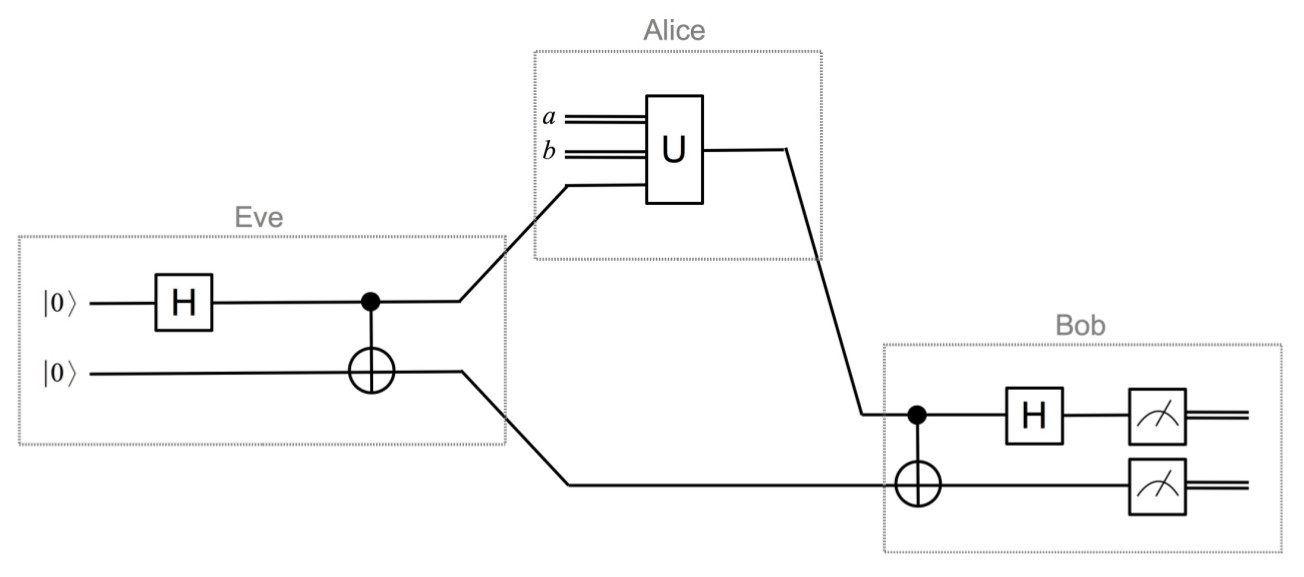
\includegraphics[scale=0.38]{superdenso.jpg}
\caption{Código Superdenso}
\label{fig:superdense}
\end{figure}


%%%%%%%%%%%%% Escolha das ferramentas
\chapter{Escolha das ferramentas}
\thispagestyle{empty} 


Neste capítulo falaremos sobre as opções e escolhas de linguagem, biblioteca e frameworks para desenvolvimento do projeto. 

\section{Linguagem}

Python foi a escolha por possuir todos os requisitos necessários para o desenvolvimento do projeto, frameworks de desenvolvimento web e bibliotecas de circuitos quânticos. Além disso, ela é vastamente utilizada em diversas aplicações e empresas como YouTube, Google, Industrial Light e Magic~\cite{pythonquotes} o que adiciona mais valor ao seu aprendizado.

\section{Biblioteca}

Tendo em vista que escolhemos Python como linguagem, precisamos definir alguma biblioteca para auxílio com os cálculos de cicuito quântico. A seguir falamos sobre algumas opções encontradas e qual foi a escolhida.
\subsection{PyQu}
PyQu é um módulo de extensão para Python 3 com o objetivo principal de providenciar um completo conjunto de tipos de dados e funções para simular computação quântica com uma sintaxe pura. Entretanto o último commit feito foi há 7 anos o que nos fez entender que o projeto foi descontinuado, fazendo com que descartássemos essa opção~\cite{pyqu}.

\subsection{Qitensor}
Qitensor, outro módulo que essencialmente é um pacote para Numpy~\cite{numpy}, utiliza semânticas mais úteis para mecânica quântica de dimensões finitas de muitas partículas. Infelizmente essa biblioteca também não recebia atualizações há mais de um ano~\cite{qitensor}.
\subsection{Qubiter}
Qubiter tem como intuito ajudar no designer e simulação de circuitos quânticos em computadores clássicos. É um projeto gêmeo do Quantum Fog e eles esperam que um dia haja uma interação entre o Quantum Fog e o Qubiter para realizar algumas tarefas, como compilação e simulação quântica~\cite{qubiter}.	

\subsection{QuTiP}
QuTiP teve sua primeira versão em Julho de 2011~\cite{qutipchangelog}. É um software open-source para simular as dinâmicas de um sistema quântico aberto que utiliza os pacotes numéricos Numpy, Scipy e Cython. Teve sua primeira versão em Julho de 2011. Possui também um output gráfico provido pela Matplotlib. QuTiP tem como objetivo providenciar simulações numéricas eficientes e amigáveis para o usuário de um variado número de Hamiltonianas comumente achadas em uma vasta quantidade de aplicações físicas. Está disponível sem custos para Linux, Mac OSX e Windows, sendo esta última com algumas restrições~\cite{qutip.org}.

\subsection{Escolhida}
QuTip foi a escolhida por possuir pacotes numéricos e também output gráfico, mesmo que, este último não tenha sido utilizado no projeto. Além de possuir a melhor documentação dentre as bibliotecas pesquisadas, com exemplos e tutoriais, ele possui funcionalidades que podem auxiliar no desenvolvimento e em trabalhos futuros.

\section{Framework Web}
Frameworks web são projetados para dar suporte no desenvolvimento de sites dinâmicos, aplicações web e web services, auxiliando no trabalho de tarefas comuns como, controle de sessão, validação de dados, acesso ao banco de dados, templates, tratamento de requisições e respostas HTTP. Dentre os frameworks web existentes para Python avaliamos neste trabalho Flask, Pyramid e Django.
\subsection{Flask}
Flask é o framework mais recente encontrado, foi criado em meados de 2010. Evoluiu muito a partir da análise de frameworks anteriores e tem se destacado em pequenos projetos. A sua comunidade é pequena comparada a do Django mas é ativa em listas de e-mail e no IRC~\cite{ryanbrown}. 

\subsection{Pyramid}
O Pyramid foi criado a partir do projeto Pylons~\cite{pylonsproject} e recebeu o nome de Pyramid somente no ano de 2010, mesmo tendo sua primeira release em 2005. É um framework tão maduro quanto o Django e disponibiliza mais flexibilidade para desenvolvedores que possuem projetos onde o caso de uso não se encaixe muito bem nos padrões do mapeamento objeto-relacional, que nada mais é do que a representação das tabelas do banco de dados através de classes onde cada resgistro é representado como uma instancia da classe~\cite{pyramid}. Pode-se dizer que Pyramid é o framework mais flexível dentre os estudados. Apesar disso, pareceu muito mais complexo do que nosso projeto necessitava. Além disso, ele possui a comunidade mais inativa dentre os frameworks pesquisados.

\subsection{Django}
Django foi lançado em 2005. É um framework com foco em grandes aplicações que inclui dezenas de extras para lidar com as tarefas comuns do desenvolvimento web, como por exemplo autenticação e administração de conteúdo, além de auxiliar também com questões de segurança como SQL injection com seus querysets, evitar ataques Cross Site Scripting e fornecer proteção a Clickjacking~\cite{django}. Sem dúvida o Django é o framework mais popular e a lista de sites que o utilizam é impressionante, tendo mais de 5000 páginas~\cite{listadjangosites}. Para sites que possuem requisitos comuns, Django segue padrões bem sensatos tornando-o uma escolha bem popular entre aplicações web de porte médio ou grande.

\subsection{Comunidade}
Django possui uma quantidade enorme de perguntas no StackOverflow se comparado com os outros dois Frameworks, Django 144.000, Flask 16.600, Pyramid 1.900 (Maio 2017)~\cite{stackoverflowtags}. Já no Github Flask e Django têm números semelhantes e Pyramid 10 vezes menos, Flask possui um pouco mais de 27.200 estrelas, Django pouco mais de 25.900 e Pyramid 2.300~\cite{github}. Esses números evidenciam a populariedade e o suporte oferecido por cada framework.

\subsection{Escolhido}
O Flask seria uma boa opção entretanto escolhemos o Django por:
\begin{itemize}
\item possuir uma grande comunidade ativa;
\item diversas ferramentas já inclusas, evitando o tempo de reprogramação de funções comuns;
\item ser facilmente escalável, pensando em uma futura continuação deste Projeto Final
\item ser uma ferramenta muito utilizada no mercado, trazendo mais benefícios com o aprendizado.
\end{itemize}


%%%%%%%%%%%%%%% Desenvolvimento
\chapter{Desenvolvimento e Resultados}
\thispagestyle{empty} 

O simulador deveria ter uma área com inputs de tempo, portas e o circuito. Primeiramente, definimos a interface geral, determinando onde seria localizada cada funcionalidade. Como um dos objetivos do projeto é simular o tempo que um computador quântico levaria para executar o circuito, decidimos por colocar os inputs em local de destaque, ficando assim à esquerda e a cima. Resolvemos que as portas ficariam também a cima, pois ao carregar a página o circuito estaria vazio e assim, ela se diferenciaria dos inputs ficando à direita. Por final, precisamos de uma área para mostrar o resultado do circuito que foi deixado abaixo de tudo pois ela seria dependente das anteriores. Também adicionamos abaixo do circuito, botões para exemplificar o código superdenso, descrito na seção \ref{sec:superdenso} para facilitar os testes e uso inicial do simulador. Na Figura~\ref{fig:simulador} pode ser visto uma captura de tela do simulador, que pode ser acessado em \url{https://demo-quantum.herokuapp.com/simulador/}.

\begin{figure}[H]
\centering
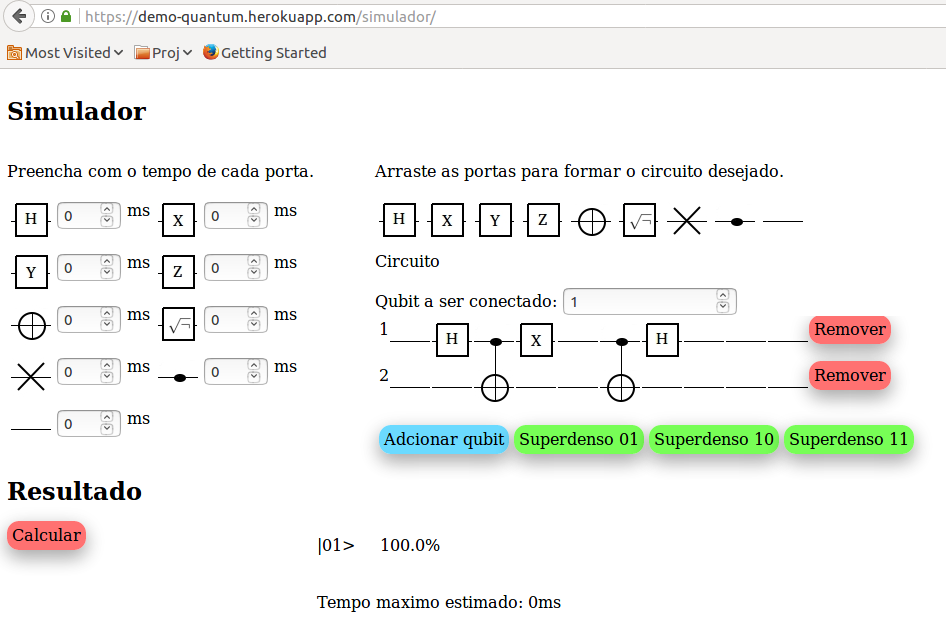
\includegraphics[scale=0.5]{simulador-pagina.png}
\caption{Nosso simulador circuito quântico online}
\label{fig:simulador}
\end{figure}

\section{Arquitetura}

Escolhemos o padrão Model-View-Controller (MVC) para o projeto já que é o modelo padrão seguido pelo Django e que faz muito sentido para o desenvolvimento de aplicações online.

Esse estilo arquitetural é composto de três elementos: modelo, visão e controle, ilustrados na Figura~\ref{fig:mvc}. O modelo é composto dos elementos que representam os principais conceitos do domínio, se pensarmos na orientação a objetos, o modelo seriam as classes do sistema e que normalmente são persistidas em bancos de dados, mas não possuem nenhum acesso de fora do sistema. Já a visão é composta por elementos de interface com o usuário, podendo ser uma interface gráfica, linha de comando ou uma API que manipulam elementos do modelo. E por último, o controle são os elementos responsáveis pela orquestração, que manipulam uma visão e executam os casos de uso.

No MVC uma visão conhece seu modelo mas o modelo não conhece sua visão, os controles conhecem suas visões mas a visão não conhece seu controle. E as entidades do modelo não conhecem ninguém a não ser as outras entidades do modelo.

\begin{figure}[H]
\centering
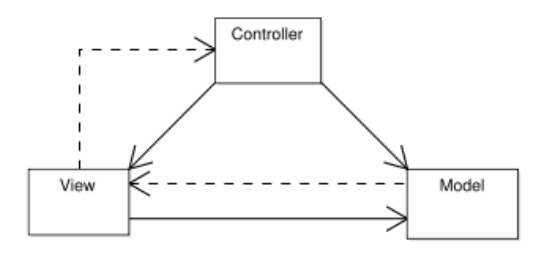
\includegraphics[scale=0.4]{mvc.png}
\caption{Diagrama MVC \cite{mvc-murta}}
\label{fig:mvc}
\end{figure}

Vantagens do MVC:
\begin{itemize}
\item responsabilidades bem definidas por componente
\item modularização da aplicação, o que traz independência 
\item fácil manutenabilidade
\item alta reutilização
\item possibilita desenvolvedores trabalharem simultaneamente
\end{itemize}

O Django possui uma particulares, ele utiliza o padrão Model View Controller (MVC), entretanto possui nomes peculiares para seus componentes. Ele renomeia a \textit{view} para \textit{template} e o \textit{controller} para \textit{view}, o que gera confusão e reclamações de muitos usuários. No próprio site do Django~\cite{django} existe uma pergunta sobre isso onde eles respondem que \textit{view} representa os dados que são apresentados ao usuário, não necessariamente como é apresentado. Então para eles a \textit{view} representa qual informação é vista e \textit{template} como ela é vista~\cite{django-mvc}.

\section{Drag and Drop} \label{sec:dragdrop}

Como o simulador deveria ser amigável para o usuário decidimos utilizar Drag \& Drop (D\&{D}) para a criação/edição do circuito. Resolvemos que o simulador deveria ter uma área com as portas quânticas disponíveis para montar o circuito quântico e a partir dessa área o usuário poderia arrastar as portas para formar o circuito. Entretanto os D\&{D} convencionais apenas possibilitavam o arrastar de um elemento para um outro container, ou seja, o elemento deixava de existir no container original e era adicionado no final. O que queríamos era que o elemento inicial continuasse existindo onde estava e que uma cópia do mesmo fosse criada e adicionada ao container alvo, por isso foi necessário implementar o nosso próprio.

Sendo assim utilizamos Javascript(JS) e JQuery~\cite{jquery}, uma biblioteca de JS, para criar uma cópia do elemento que sofreu o evento de Drag e movemos a cópia até o destino do Drop. Ao realizar o Drop existe uma checagem para excluir o elemento existente e adicionar a cópia. Nos materiais encontrados sobre D\&{D} o elemento utilizado pelo Javascript para capturar o elemento do drop era o ev.target o que gera alguns problemas já que esse target não traz especificamente o elemento com o evento de drop atrelado, podendo trazer uma das divs que o encapsulam ou algum outro elemento mais interno fazendo com que não houvesse uma consistência do retorno. Para resolver esse problema decidimos utilizar currentTarget ao invés do target.

Quando pensamos nas portas de 2 qubits nos deparamos com outro problema, o de a seleção do qubit de controle. A escolha foi ter um input que serviria de alvo do segundo qubit, fazendo o tratamento para quando o alvo era igual ao bit do Drop ou caso o alvo fosse maior que o número de bits. No primeiro caso é solto um alerta com a mensagem de que não é possível arrastar a porta para o mesmo bit alvo da conexão, e no segundo caso o alvo se torna o último qubit do circuito ou o primeiro, caso o valor seja negativo.

\section{Cálculo via AJAX}

AJAX, ou JavaScript e XML assíncronos, não é uma linguagem e sim uma combinação de técnicas que utilizam ferramentas já embutidas do browser para realizar requisições ao servidor e receber respostas do mesmo de forma assíncrona, sem a necessidade de recarregar a página inteira, apenas parte dela.

A escolha do AJAX para realização do cálculo se deve ao simples fato de que o simulador tem o intuito de ser amigável ao usuário e dessa forma utilizando AJAX não existe a necessidade de recarregar a página ou ser direcionado para uma outra, o que é uma funcionalidade muito útil para o nosso sistema.

Primeiramente, existe o tratamento do circuito para um objeto de fácil acesso à aplicação onde decidimos utilizar um JSON (JavaScript Object Notation - Notação de Objetos JavaScript) que é uma formatação de dados de fácil leitura e escrita para pessoas e de fácil interpretação e geração por computadores. JSON é composto por duas estruturas: uma coleção de pares nome/valor e uma lista ordenada de valores.

Por serem estruturas de dados comuns a todas as linguagens, de formato para troca de dados para nosso sistema foi decidido como uma boa opção~\cite{json}.

Após isso colocamos os elementos (as portas pertencentes ao circuito) em um array de arrays. Também colocamos a quantidade de qubits que o circuito possui, as conexões entre as portas e enviamos para o servidor.

No servidor, por estarmos utilizando o Django, o tratamento de requisição e respostas já é realizado~\cite{django-req-resp}. Dentro da view, que é considerado um controle pelo Django, bastou receber o objeto Request, fazer a leitura do JSON que foi enviado pelo AJAX e trabalhar em cima dele utilizando a biblioteca QuTip para realizar o cálculo.

A parte do cálculo do tempo, por não necessitar da biblioteca ou qualquer outra informação por parte do servidor, pode ser feita na própria página pelo JavaScript, pois as únicas informações necessárias são os inputs de tempo de cada porta e quais portas formavam o circuito.

Ao receber o retorno do servidor, o AJAX adiciona os resultados, tanto do cálculo do circuito quanto do cálculo do tempo, na área do HTML de resultados da página.

\section{Usando QuTip}

Utilizar a biblioteca QuTip se mostrou um desafio maior do que inicialmente previsto. Entretanto, após o período de familiarização inicial, ela se tornou uma excelente ferramenta. QuTip possui um objeto, o QubitCircuit, que representa um programa ou algoritmo quântico que mantém uma sequência de portas (chamados \textit{Gates}). O QubitCircuit possui uma função add\_gate com os seguintes parâmetros:
\begin{itemize}
\item gate - Nome da porta, dentro de uma lista aceitável. RX, RY, RZ, CRX, CRY, CRZ, SQRTNOT, SNOT, PHASEGATE, CPHASE, CNOT, CSIGN, BERKELEY, SWAPalpha, SWAP, ISWAP, SQRTSWAP, SQRTISWAP, FREDKIN, TOFFOLI, GLOBALPHASE;
\item targets - Uma lista com os qubits alvos;
\item controls - Uma lista com os qubits de controle;
\item arg\_value - Parâmetro para a transformação, do tipo Float;
\item arg\_label - Label para representação da porta.
\end{itemize}

Dependendo da porta desejada, alguns dos parâmetros são obrigatórios. Por exemplo, para adicionar a porta Hadamard basta qcircuit.add\_gate(``SNOT'', targets=[0]), onde os parâmetros obrigatórios são \textit{gate} e \textit{targets}.

Após montarmos o objeto QubitCircuit com as portas passadas no Request, deve-se calcular a matriz de propagação utilizando a função QubitCircuit.propagators() que faz esse cálculo. Ela retorna uma lista com os passos em forma de matrizes unitárias operando da esquerda para a direita. Com essa lista é possível chamar a função gate\_sequence\_product() que retorna a matriz unitária final.

O objeto gerado pela função gate\_sequence\_product() é então multiplicado pelo vetor coluna dos qubits passados no input que inicialmente são sempre iguais a $\ket{0}$. Essa multiplicação gera um novo vetor coluna com as probabilidades dos valores finais para o circuito e é nesse vetor que é feito uma análise para retirada legível dos resultados que finalmente são retornados para o AJAX.

\section{Hospedagem - Heroku}

Como o simulador tem o objetivo de ser online utilizamos a plataforma da nuvem Heroku para a hospedagem. O Heroku é um PaaS (Platform as a Service) que faz com que o desenvolvedor não tenha que se preocupar com infraestrutura tendo assim foco total no desenvolvimento, sem precisar gerenciar, fazer a manutenção e garantir a segurança do servidor~\cite{heroku}. Ele possui uma opção grátis que dá suporte a diversas linguagem sendo uma delas Python, o que fez dela uma boa escolha.

A configuração do projeto para rodar no Heroku não é complicada. Basta colocar o projeto no Git, preparar um ambiente virtual com todas as dependências necessárias, gerar um arquivo texto chamado ``requirements.txt'' com essas dependências, o que pode ser feito com o comando ``pip freeze > requirements.txt'' e adicionar esse arquivo ao diretório do projeto. Devemos também criar um outro arquivo ``runtime.txt'' para especificar a versão do Python sendo utilizada. É necessário criar um ``Procfile'' que serve para declarar o comando que será executado para começar a aplicação. No caso do nosso projeto colocamos ``web: gunicorn quantum-circuit-simulator.wsgi --log-file -''.

Após essas configurações básicas é necessário criar uma conta no Heroku e instalar o Heroku CLI. Com a instalação do Heroku CLI podemos executar o comando ``heroku login'' e entrar com as credenciais de login. Após isso, criar uma aplicação com o comando ``heroku create nome-aplicacao'', adicionar todas as alterações feitas no projeto e realizar o deploy da aplicação no Heroku ``git push heroku master''.

Durante o deploy o Heroku detecta a linguagem, faz a instalação dos requisitos que estão no arquivo ``requirements.txt'' e roda o comando no Procfile.

Com o deploy da sua aplicação feito basta acessar a url da aplicação acessando sua conta do Heroku ou executando o comando ``heroku open''~\cite{heroku-python}.

\section{Resultados}

O projeto alcançou o objetivo traçado ao criar um simulador web de circuito quântico. O código gerado se encontra no GitHub: \url{https://github.com/iblackman/quantum-circuit-simulator}.

Na Figura~\ref{fig:resHtml} podemos ver uma parte do código HTML produzido, que cria a área dos inputs de tempo das portas, as portas a serem arrastadas, o circuito e a parte onde é mostrado o resultado.

\begin{figure}[H]
\centering
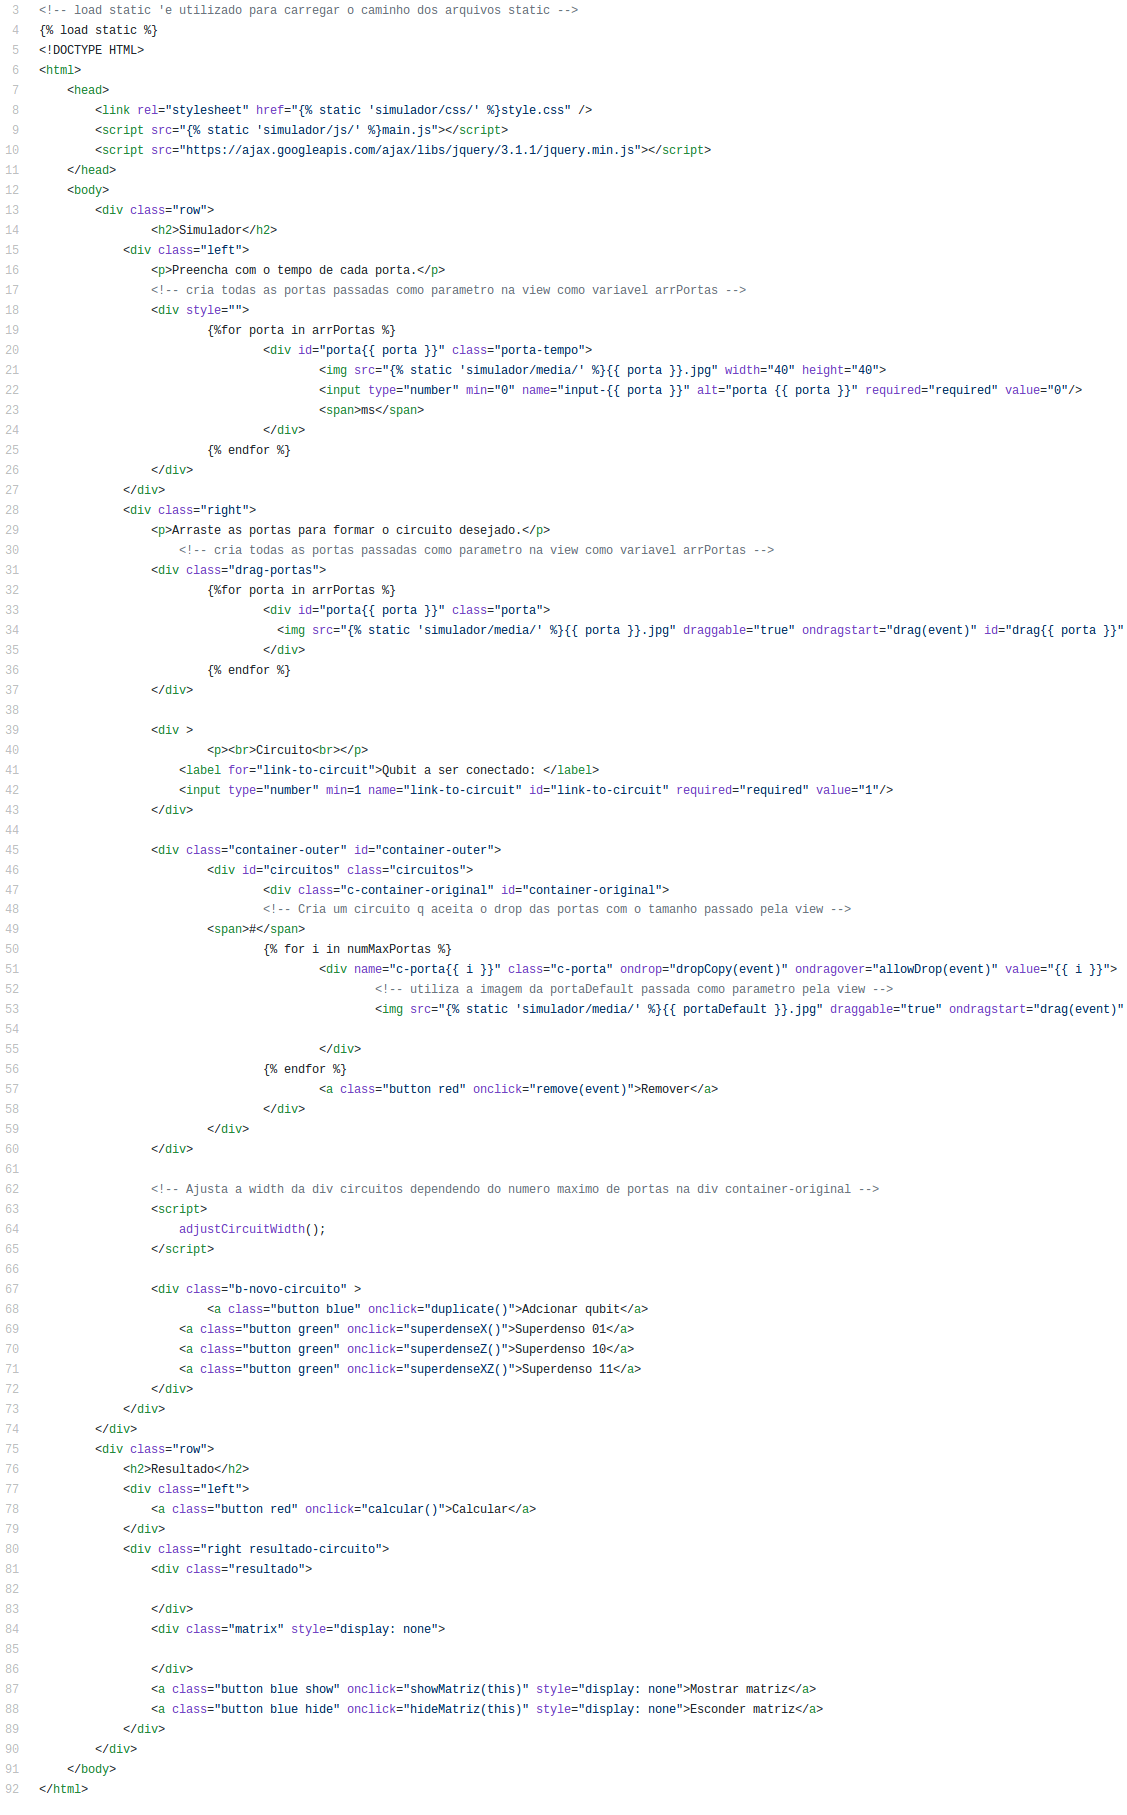
\includegraphics[scale=0.35]{index.png}
\caption{Parte do HTML}
\label{fig:resHtml}
\end{figure}

Já na Figura~\ref{fig:resJavascript} podemos ver uma parte do código Javascript com a função de \textit{Drop} criada, como descrito na seção~\ref{sec:dragdrop}.

\begin{figure}[H]
\centering
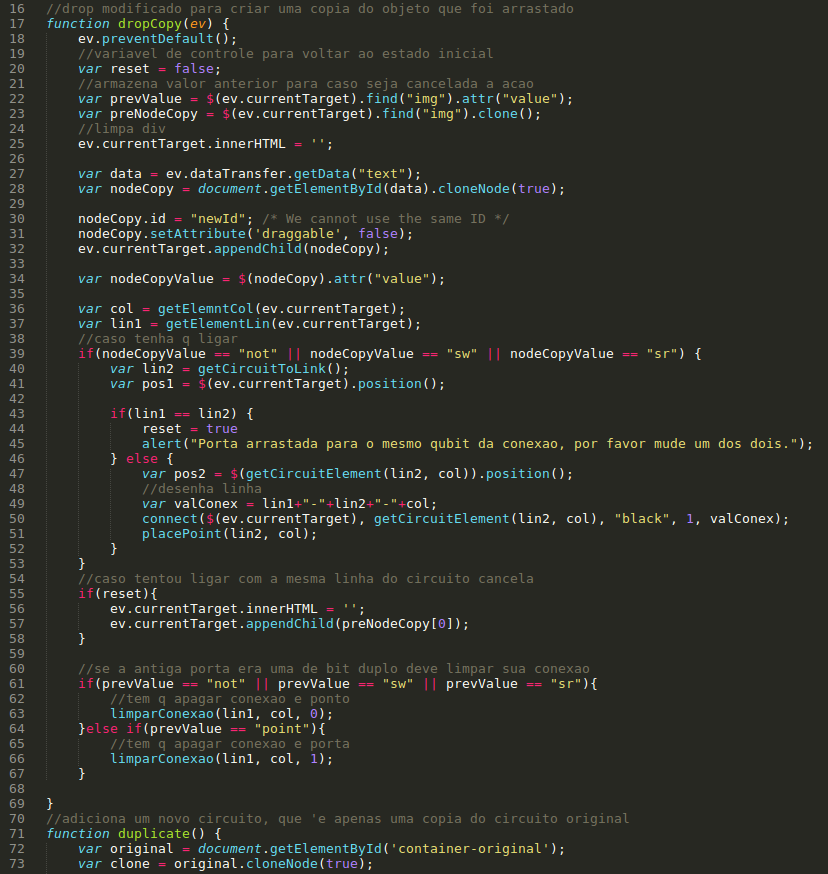
\includegraphics[scale=0.43]{javascript.png}
\caption{Parte do Javascript}
\label{fig:resJavascript}
\end{figure}

Finalmente, na Figura~\ref{fig:resPython} está sendo ilustrado uma parte do código Python que faz o cálculo do circuito quântico montado, gerando o resultado do qubit final.

\begin{figure}[H]
\centering
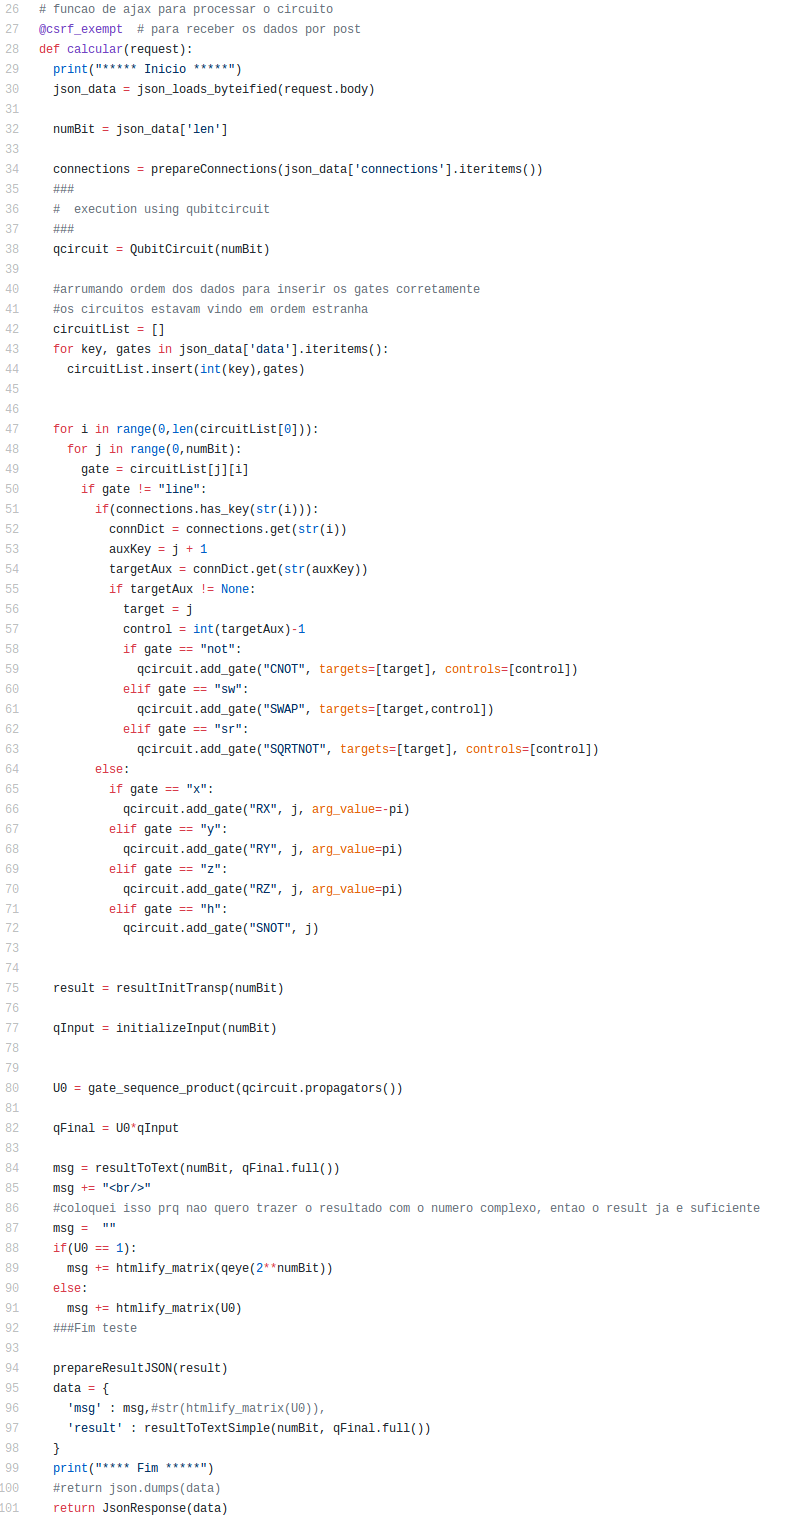
\includegraphics[scale=0.40]{view.png}
\caption{Parte do programa em Python}
\label{fig:resPython}
\end{figure}

\chapter{Conclusão e Trabalhos Futuros}
\thispagestyle{empty} 

O trabalho teve como objetivo a implementação de um simulador de circuitos quânticos que executa algoritmos quânticos em um computador clássico, recebendo alguns valores de entrada para estimar o tempo gasto por cada porta quântica. Assim, o simulador consegue emular o que seria obtido em um computador quântico caso ele seja construído emulando sobreposição de estados e entrelaçamento. O simulador dispões de algumas funcionalidades como arraste das portas para a construção do circuito, criação de circuitos já preparados, além de disponibilidade online. Isso tudo com o intuíto de facilitar a interação com o usuário.

O projeto providenciou um enorme aprendizado em duas áreas que não estão relacionadas e que não são obrigatórias na grade curricular do aluno, Computação Quântica e Desenvolvimento Web. Na parte do desenvolvimento web tivemos a oportunidade de estudar a linguagem de programação Python e um de seus Frameworks para desenvolvimento web, o Django, e realizar deploy na plataforma na nuvem Heroku. E quanto a parte de computação quântica estudamos a biblioteca QuTip para realização dos cálculos além dos algoritmos quânticos e seu funcionamento. 

Como trabalhos futuros pode-se implantar novas portas, melhora do sistema de Drag and Drop principalmente no caso das portas de dois qubits, melhora no design do simulador com a ideia de torná-lo mais atrativo ao usuário, e alterar a forma como os resultados são mostrados para facilitar o entendimento do usuário. O sistema pode ser expandido, adicionando novas funcionalidades como leitura de um circuito a partir de algum tipo de arquivo, e a possibilidade de salvar um circuito já montado.

%%%%%%%%%%%%%%%%%%%%%%%%%%%%%%%%%%%%%%%%%%%%%%%%%%%%%    REFERÊNCIAS BIBLIOGRÁFICAS
\bibliographystyle{plain}
\bibliography{monografia}



\end{document}


